\documentclass[11pt]{article}

% ---------- Packages ----------
\usepackage[margin=1in]{geometry}
\usepackage{lmodern}
\usepackage[T1]{fontenc}
\usepackage[utf8]{inputenc}
\usepackage{microtype}
\usepackage{titlesec}
\usepackage{enumitem}
\usepackage{tabularx}
\usepackage{multicol}
\usepackage{graphicx}
\usepackage[dvipsnames,svgnames,x11names]{xcolor}
\usepackage{tikz}
\usepackage{tcolorbox}
\tcbuselibrary{most}
\usepackage{fancyhdr}
\usepackage{listings}
\usepackage{pifont}
\usepackage{hyperref} % keep near end

% TikZ libs
\usetikzlibrary{arrows.meta,positioning,shadows,shadows.blur}

\hypersetup{colorlinks=true, linkcolor=black, urlcolor=blue, citecolor=black}

% ---------- Colors ----------
\definecolor{ink}{RGB}{26,26,26}
\definecolor{accent}{RGB}{47,117,212}
\definecolor{accent2}{RGB}{42,157,143}
\definecolor{warn}{RGB}{224,93,68}
\definecolor{ok}{RGB}{33,150,83}
\definecolor{sun}{RGB}{253,187,45}
\definecolor{panel}{RGB}{245,247,250}
\definecolor{shadow}{RGB}{210,217,226}
\definecolor{lav}{RGB}{120,94,240}
\definecolor{slate}{RGB}{100,116,139}
\definecolor{lststring}{rgb}{0.925,0.282,0.600} % Custom color for code strings

% ---------- Fonts / sectioning ----------
\titleformat{\section}{\Large\bfseries\color{ink}}{\thesection}{1em}{}
\titleformat{\subsection}{\large\bfseries\color{ink}}{\thesubsection}{0.75em}{}
\titleformat{\subsubsection}{\bfseries\color{ink}}{\thesubsubsection}{0.5em}{}
\setlist[itemize]{leftmargin=1.2em}
\setlist[enumerate]{leftmargin=1.2em}

% ---------- Fancy header/footer ----------
\pagestyle{fancy}
\fancyhf{}
\lhead{\textbf{SIRUS Rails for BLT}}
\rhead{\thepage}
\cfoot{\color{slate}\footnotesize Serve people. Build trustworthy scaffolding. Keep the tail honest. Move.}
\setlength{\headheight}{14pt}

% ---------- TikZ styles ----------
\tikzset{
  box/.style={
    rectangle,draw,rounded corners,align=center,inner sep=3pt,
    text width=3.6cm
  },
  n/.style={
    rounded corners, draw=accent, fill=panel, align=center, inner sep=3pt,
    blur shadow={shadow xshift=1ex, shadow yshift=-1ex, shadow blur steps=5},
    text width=3.4cm
  },
  svc/.style={
    rounded corners, draw=accent, fill=panel, align=center, inner sep=6pt,
    blur shadow={shadow xshift=1ex, shadow yshift=-1ex, shadow blur steps=5},
    text width=3.6cm
  },
  edge/.style={->, thick}
}

% ---------- tcolorbox styles ----------
\tcbset{
  enhanced,
  frame code={\path[fill=shadow] ([xshift=2pt,yshift=-2pt]frame.north west) rectangle (frame.south east);},
  coltitle=ink,
  colback=panel,
  colframe=accent,
  boxrule=0.6pt,
  arc=3pt,
  outer arc=3pt,
  top=6pt,bottom=6pt,left=8pt,right=8pt,
  toptitle=4pt,bottomtitle=2pt,
  title style={font=\bfseries\large},
  colbacktitle=panel
}

% Titles wrapped in braces so commas/colons are safe
\newtcolorbox{panelA}[2][]{title={#2}, #1}
\newtcolorbox{panelB}[2][]{title={#2}, colframe=accent2, #1}
\newtcolorbox{panelC}[2][]{title={#2}, colframe=lav, #1}
\newtcolorbox{panelWarn}[2][]{title={#2}, colframe=warn, #1}
\newtcolorbox{callout}[1][]{colback=white, colframe=accent, arc=6pt, boxrule=0.8pt, #1}

% ---------- Listings (code) ----------
\lstdefinestyle{code}{%
  basicstyle=\ttfamily\small,
  keywordstyle=\color{lav}\bfseries\relax,
  stringstyle=\color{lststring}\relax,
  commentstyle=\color{slate}\itshape\relax,
  showstringspaces=false,
  breaklines=true,
  frame=single,
  rulecolor=\color{shadow},
  numbers=left,
  numberstyle=\tiny\color{slate},
  xleftmargin=1.5em,
  framexleftmargin=1.2em,
  inputencoding=utf8
}
\lstset{style=code}

\lstdefinelanguage{json}{
  string=[s]{"}{"}, % All strings are between quotes
  commentstyle=\color{slate},
  keywordstyle=\color{lav}\bfseries,
  morekeywords={true,false,null}, % JSON keywords
  showstringspaces=false,
  breaklines=true,
}

% ---------- Convenience ----------
\newcommand{\cmark}{\textcolor{ok}{\ding{51}}}
\newcommand{\xmark}{\textcolor{warn}{\ding{55}}}

% ---------- Title ----------
\begin{document}
\begin{center}
{\huge \textbf{SIRUS Rails for BLT}}\\[4pt]
{\large \textit{A Visual, Intuitive, Comic-Style Guide for Safe, Auditable AI}}\\[6pt]
\textcolor{slate}{\small \textbf{Vow:} Serve people. Build trustworthy scaffolding. Keep the tail honest. Move.}\\[10pt]
\end{center}

% ---------- Opening Spread ----------
\begin{panelA}{The Whole Picture (One-Page Intuition)}
\begin{minipage}{0.60\textwidth}
\textbf{Why this exists.} Modern ML needs rails. SIRUS provides governance-as-love: Safety, Integrity, Reproducibility, Utility, Stewardship. BLT (HPC at Lewis \& Clark) gives us the horsepower. Together, we can move fast \emph{and} keep the tail honest.

\medskip
\textbf{The loop:}
\begin{enumerate}
  \item \textbf{Ingest} only public or licensed data $\rightarrow$ create a \textbf{Dataset Receipt}.
  \item \textbf{Freeze} the environment $\rightarrow$ \textbf{EnvLock}.
  \item \textbf{Assemble} the job manifest $\rightarrow$ \textbf{Pack}.
  \item \textbf{Preflight} on BLT (Parsl hook) $\rightarrow$ jobs without Pack/EnvLock \textbf{fail closed}.
  \item \textbf{Ledger} writes a tamper-evident \textbf{Receipt}.
  \item \textbf{Safety gates} (DP, red-team, evals) $\rightarrow$ \textbf{TailContracts} auto-remedy if tripped.
  \item \textbf{Publish} DP-safe aggregates to the \textbf{Hope Ledger}. Invite external audit.
\end{enumerate}
\end{minipage}\hfill
\begin{minipage}{0.38\textwidth}
\centering
\resizebox{\linewidth}{!}{%
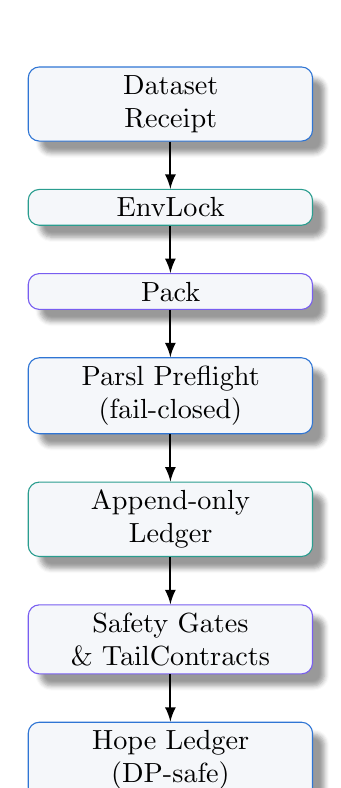
\begin{tikzpicture}[>=latex, node distance=6mm]
\node[n] (ingest) {Dataset\\Receipt};
\node[n, below=of ingest, draw=accent2] (env) {EnvLock};
\node[n, below=of env, draw=lav] (pack) {Pack};
\node[n, below=of pack, draw=accent] (pre) {Parsl Preflight\\(fail-closed)};
\node[n, below=of pre, draw=accent2] (ledger) {Append-only\\Ledger};
\node[n, below=of ledger, draw=lav] (safety) {Safety Gates\\\& TailContracts};
\node[n, below=of safety, draw=accent] (hope) {Hope Ledger\\(DP-safe)};
\draw[->, thick] (ingest) -- (env);
\draw[->, thick] (env) -- (pack);
\draw[->, thick] (pack) -- (pre);
\draw[->, thick] (pre) -- (ledger);
\draw[->, thick] (ledger) -- (safety);
\draw[->, thick] (safety) -- (hope);
\end{tikzpicture}
}%
\end{minipage}
\end{panelA}

% ---------- Cast of Characters ----------
\begin{panelB}{Cast of Characters (Who Does What)}
\begin{multicols}{2}
\begin{itemize}
  \item \textbf{Data Steward} — verifies licenses/consent; signs Dataset Receipts.
  \item \textbf{Safety Officer} — runs evals, red-team, DP checks; triggers remedies.
  \item \textbf{Infrastructure Owner} — maintains ledger, keys, preflight.
  \item \textbf{PRR Quorum} — approves high-risk changes; holds well-being gate.
  \item \textbf{External Auditor} — independent review of receipts and process.
\end{itemize}
\columnbreak
\begin{callout}
\textbf{Plain language promise (for non-technical stakeholders).}\\
Every job carries its paperwork. No paperwork, no run. If a safety gate trips, we automatically slow down, fix it, and leave a trail you can verify.
\end{callout}
\end{multicols}
\end{panelB}

% ---------- SIRUS Rails ----------
% ---------- SIRUS Rails ----------
\begin{panelC}{The Rails}
	\begin{multicols}{2}
		\textbf{1) Dataset Receipts}\\[-4pt]
		\begin{itemize}
			\item Source URI, license \& consent statement
			\item File hashes, OCR/redaction logs
			\item Steward identity \& signature
		\end{itemize}
		
		\textbf{3) Pack}\\[-4pt]
		\begin{itemize}
			\item Ties receipts + code commit + EnvLock
			\item Allowed environments (e.g., BLT Parsl cfg)
			\item Governance signatures (M-of-N)
		\end{itemize}
		
		\textbf{5) Ledger \& Hope Ledger}\\[-4pt]
		\begin{itemize}
			\item Append-only receipts for every run
			\item DP-safe public aggregates (no raw PII)
			\item Audit hooks \& external review
		\end{itemize}
		
		\columnbreak
		
		\textbf{2) EnvLock}\\[-4pt]
		\begin{itemize}
			\item Container digest, OS image, lockfiles
			\item Hardware fingerprint (optional)
			\item Signed snapshot of what will run
		\end{itemize}
		
		\textbf{4) TailContracts}\\[-4pt]
		\begin{itemize}
			\item Triggers \& remedies (freeze, revoke keys)
			\item Restoration-first discipline
			\item Human-readable + machine-enforced
		\end{itemize}
	\end{multicols}
\end{panelC}

% ---------- BLT Integration Diagram ----------
\begin{panelA}{How It Fits on BLT (Parsl + SGE)}
\begin{center}
\resizebox{\linewidth}{!}{%
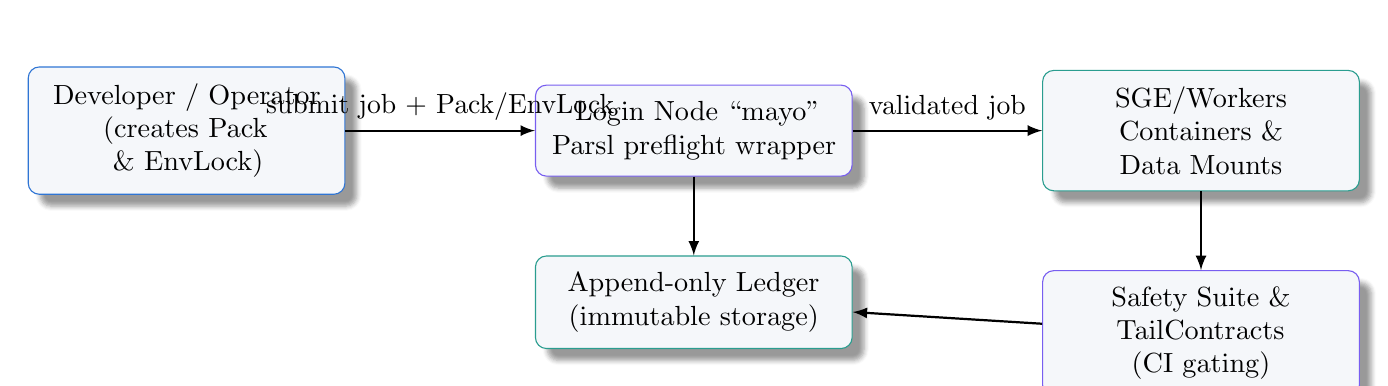
\begin{tikzpicture}[>=latex, node distance=10mm]
\node[svc] (user) {Developer / Operator\\(creates Pack \& EnvLock)};
\node[svc, right=of user, xshift=4em, draw=lav] (mayo) {Login Node ``mayo''\\Parsl preflight wrapper};
\node[svc, right=of mayo, xshift=4em, draw=accent2] (sge) {SGE/Workers\\Containers \& Data Mounts};
\node[svc, below=of mayo, draw=accent2] (ledger) {Append-only Ledger\\(immutable storage)};
\node[svc, below=of sge, draw=lav] (safety) {Safety Suite \& TailContracts\\(CI gating)};
\draw[edge] (user) -- node[above]{submit job + Pack/EnvLock} (mayo);
\draw[edge] (mayo) -- node[above]{validated job} (sge);
\draw[edge] (mayo) -- (ledger);
\draw[edge] (sge) -- (safety);
\draw[edge] (safety) -- (ledger);
\end{tikzpicture}
}%
\end{center}
\end{panelA}

% ---------- Preflight Rule ----------

% 

% ---------- Final Notes ----------
\begin{callout}
\textbf{Final Notes.} This guide is intentionally visual, concise, and fail-closed. If something feels unsafe or unclear, stop, document, and ask the governance body to review before proceeding.
\end{callout}

\vspace{1ex}
\noindent\textit{This document intentionally avoids guidance for secrecy, covert operations, or unlicensed data use. It is designed to help demotivated readers \emph{see} the system and regain curiosity through concrete, visual structure.}

\end{document}